\documentclass[1p]{elsarticle_modified}
%\bibliographystyle{elsarticle-num}

%\usepackage[colorlinks]{hyperref}
%\usepackage{abbrmath_seonhwa} %\Abb, \Ascr, \Acal ,\Abf, \Afrak
\usepackage{amsfonts}
\usepackage{amssymb}
\usepackage{amsmath}
\usepackage{amsthm}
\usepackage{scalefnt}
\usepackage{amsbsy}
\usepackage{kotex}
\usepackage{caption}
\usepackage{subfig}
\usepackage{color}
\usepackage{graphicx}
\usepackage{xcolor} %% white, black, red, green, blue, cyan, magenta, yellow
\usepackage{float}
\usepackage{setspace}
\usepackage{hyperref}

\usepackage{tikz}
\usetikzlibrary{arrows}

\usepackage{multirow}
\usepackage{array} % fixed length table
\usepackage{hhline}

%%%%%%%%%%%%%%%%%%%%%
\makeatletter
\renewcommand*\env@matrix[1][\arraystretch]{%
	\edef\arraystretch{#1}%
	\hskip -\arraycolsep
	\let\@ifnextchar\new@ifnextchar
	\array{*\c@MaxMatrixCols c}}
\makeatother %https://tex.stackexchange.com/questions/14071/how-can-i-increase-the-line-spacing-in-a-matrix
%%%%%%%%%%%%%%%

\usepackage[normalem]{ulem}

\newcommand{\msout}[1]{\ifmmode\text{\sout{\ensuremath{#1}}}\else\sout{#1}\fi}
%SOURCE: \msout is \stkout macro in https://tex.stackexchange.com/questions/20609/strikeout-in-math-mode

\newcommand{\cancel}[1]{
	\ifmmode
	{\color{red}\msout{#1}}
	\else
	{\color{red}\sout{#1}}
	\fi
}

\newcommand{\add}[1]{
	{\color{blue}\uwave{#1}}
}

\newcommand{\replace}[2]{
	\ifmmode
	{\color{red}\msout{#1}}{\color{blue}\uwave{#2}}
	\else
	{\color{red}\sout{#1}}{\color{blue}\uwave{#2}}
	\fi
}

\newcommand{\Sol}{\mathcal{S}} %segment
\newcommand{\D}{D} %diagram
\newcommand{\A}{\mathcal{A}} %arc


%%%%%%%%%%%%%%%%%%%%%%%%%%%%%5 test

\def\sl{\operatorname{\textup{SL}}(2,\Cbb)}
\def\psl{\operatorname{\textup{PSL}}(2,\Cbb)}
\def\quan{\mkern 1mu \triangleright \mkern 1mu}

\theoremstyle{definition}
\newtheorem{thm}{Theorem}[section]
\newtheorem{prop}[thm]{Proposition}
\newtheorem{lem}[thm]{Lemma}
\newtheorem{ques}[thm]{Question}
\newtheorem{cor}[thm]{Corollary}
\newtheorem{defn}[thm]{Definition}
\newtheorem{exam}[thm]{Example}
\newtheorem{rmk}[thm]{Remark}
\newtheorem{alg}[thm]{Algorithm}

\newcommand{\I}{\sqrt{-1}}
\begin{document}

%\begin{frontmatter}
%
%\title{Boundary parabolic representations of knots up to 8 crossings}
%
%%% Group authors per affiliation:
%\author{Yunhi Cho} 
%\address{Department of Mathematics, University of Seoul, Seoul, Korea}
%\ead{yhcho@uos.ac.kr}
%
%
%\author{Seonhwa Kim} %\fnref{s_kim}}
%\address{Center for Geometry and Physics, Institute for Basic Science, Pohang, 37673, Korea}
%\ead{ryeona17@ibs.re.kr}
%
%\author{Hyuk Kim}
%\address{Department of Mathematical Sciences, Seoul National University, Seoul 08826, Korea}
%\ead{hyukkim@snu.ac.kr}
%
%\author{Seokbeom Yoon}
%\address{Department of Mathematical Sciences, Seoul National University, Seoul, 08826,  Korea}
%\ead{sbyoon15@snu.ac.kr}
%
%\begin{abstract}
%We find all boundary parabolic representation of knots up to 8 crossings.
%
%\end{abstract}
%\begin{keyword}
%    \MSC[2010] 57M25 
%\end{keyword}
%
%\end{frontmatter}

%\linenumbers
%\tableofcontents
%
\newcommand\colored[1]{\textcolor{white}{\rule[-0.35ex]{0.8em}{1.4ex}}\kern-0.8em\color{red} #1}%
%\newcommand\colored[1]{\textcolor{white}{ #1}\kern-2.17ex	\textcolor{white}{ #1}\kern-1.81ex	\textcolor{white}{ #1}\kern-2.15ex\color{red}#1	}

{\Large $\underline{12a_{0443}~(K12a_{0443})}$}

\setlength{\tabcolsep}{10pt}
\renewcommand{\arraystretch}{1.6}
\vspace{1cm}\begin{tabular}{m{100pt}>{\centering\arraybackslash}m{274pt}}
\multirow{5}{120pt}{
	\centering
	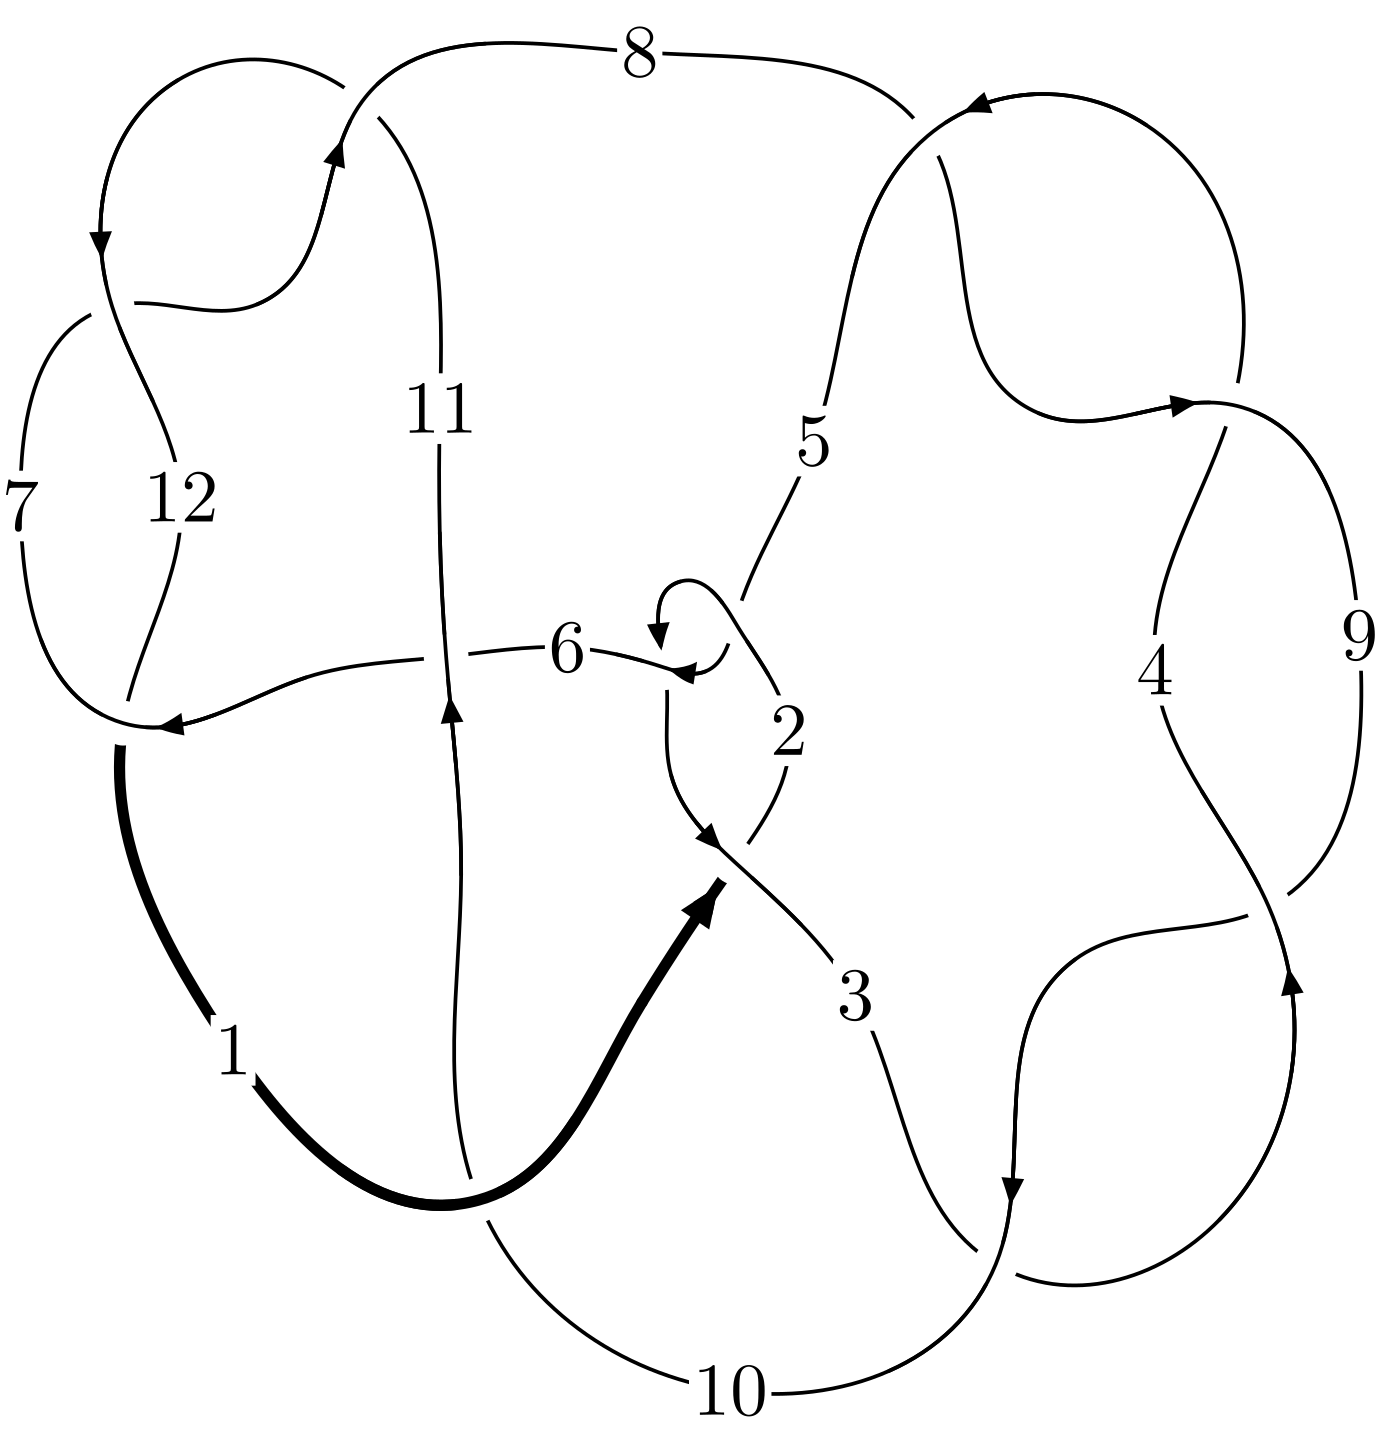
\includegraphics[width=112pt]{../../../GIT/diagram.site/Diagrams/png/1244_12a_0443.png}\\
\ \ \ A knot diagram\footnotemark}&
\allowdisplaybreaks
\textbf{Linearized knot diagam} \\
\cline{2-2}
 &
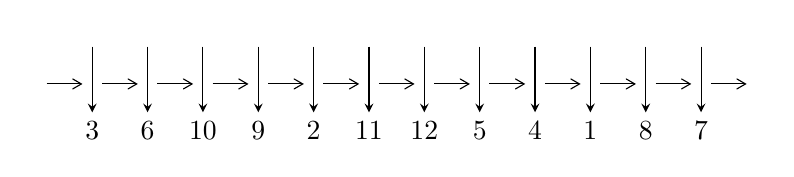
\begin{tikzpicture}[x=20pt, y=17pt]
	% nodes
	\node (C0) at (0, 0) {};
	\node (C1) at (1, 0) {};
	\node (C1U) at (1, +1) {};
	\node (C1D) at (1, -1) {3};

	\node (C2) at (2, 0) {};
	\node (C2U) at (2, +1) {};
	\node (C2D) at (2, -1) {6};

	\node (C3) at (3, 0) {};
	\node (C3U) at (3, +1) {};
	\node (C3D) at (3, -1) {10};

	\node (C4) at (4, 0) {};
	\node (C4U) at (4, +1) {};
	\node (C4D) at (4, -1) {9};

	\node (C5) at (5, 0) {};
	\node (C5U) at (5, +1) {};
	\node (C5D) at (5, -1) {2};

	\node (C6) at (6, 0) {};
	\node (C6U) at (6, +1) {};
	\node (C6D) at (6, -1) {11};

	\node (C7) at (7, 0) {};
	\node (C7U) at (7, +1) {};
	\node (C7D) at (7, -1) {12};

	\node (C8) at (8, 0) {};
	\node (C8U) at (8, +1) {};
	\node (C8D) at (8, -1) {5};

	\node (C9) at (9, 0) {};
	\node (C9U) at (9, +1) {};
	\node (C9D) at (9, -1) {4};

	\node (C10) at (10, 0) {};
	\node (C10U) at (10, +1) {};
	\node (C10D) at (10, -1) {1};

	\node (C11) at (11, 0) {};
	\node (C11U) at (11, +1) {};
	\node (C11D) at (11, -1) {8};

	\node (C12) at (12, 0) {};
	\node (C12U) at (12, +1) {};
	\node (C12D) at (12, -1) {7};
	\node (C13) at (13, 0) {};

	% arrows
	\draw[->,>={angle 60}]
	(C0) edge (C1) (C1) edge (C2) (C2) edge (C3) (C3) edge (C4) (C4) edge (C5) (C5) edge (C6) (C6) edge (C7) (C7) edge (C8) (C8) edge (C9) (C9) edge (C10) (C10) edge (C11) (C11) edge (C12) (C12) edge (C13) ;	\draw[->,>=stealth]
	(C1U) edge (C1D) (C2U) edge (C2D) (C3U) edge (C3D) (C4U) edge (C4D) (C5U) edge (C5D) (C6U) edge (C6D) (C7U) edge (C7D) (C8U) edge (C8D) (C9U) edge (C9D) (C10U) edge (C10D) (C11U) edge (C11D) (C12U) edge (C12D) ;
	\end{tikzpicture} \\
\hhline{~~} \\& 
\textbf{Solving Sequence} \\ \cline{2-2} 
 &
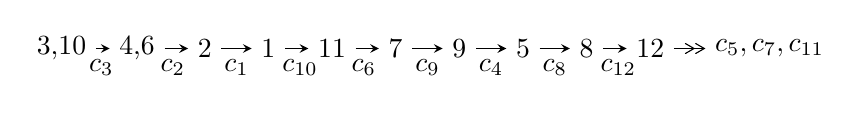
\begin{tikzpicture}[x=23pt, y=7pt]
	% node
	\node (A0) at (-1/8, 0) {3,10};
	\node (A1) at (17/16, 0) {4,6};
	\node (A2) at (17/8, 0) {2};
	\node (A3) at (25/8, 0) {1};
	\node (A4) at (33/8, 0) {11};
	\node (A5) at (41/8, 0) {7};
	\node (A6) at (49/8, 0) {9};
	\node (A7) at (57/8, 0) {5};
	\node (A8) at (65/8, 0) {8};
	\node (A9) at (73/8, 0) {12};
	\node (C1) at (1/2, -1) {$c_{3}$};
	\node (C2) at (13/8, -1) {$c_{2}$};
	\node (C3) at (21/8, -1) {$c_{1}$};
	\node (C4) at (29/8, -1) {$c_{10}$};
	\node (C5) at (37/8, -1) {$c_{6}$};
	\node (C6) at (45/8, -1) {$c_{9}$};
	\node (C7) at (53/8, -1) {$c_{4}$};
	\node (C8) at (61/8, -1) {$c_{8}$};
	\node (C9) at (69/8, -1) {$c_{12}$};
	\node (A10) at (11, 0) {$c_{5},c_{7},c_{11}$};

	% edge
	\draw[->,>=stealth]	
	(A0) edge (A1) (A1) edge (A2) (A2) edge (A3) (A3) edge (A4) (A4) edge (A5) (A5) edge (A6) (A6) edge (A7) (A7) edge (A8) (A8) edge (A9) ;
	\draw[->>,>={angle 60}]	
	(A9) edge (A10);
\end{tikzpicture} \\ 

\end{tabular} \\

\footnotetext{
The image of knot diagram is generated by the software ``\textbf{Draw programme}" developed by Andrew Bartholomew(\url{http://www.layer8.co.uk/maths/draw/index.htm\#Running-draw}), where we modified some parts for our purpose(\url{https://github.com/CATsTAILs/LinksPainter}).
}\phantom \\ \newline 
\centering \textbf{Ideals for irreducible components\footnotemark of $X_{\text{par}}$} 
 
\begin{align*}
I^u_{1}&=\langle 
-1.75431\times10^{51} u^{70}-2.70378\times10^{52} u^{69}+\cdots+3.02784\times10^{53} b+1.04182\times10^{54},\\
\phantom{I^u_{1}}&\phantom{= \langle  }4.41577\times10^{53} u^{70}+4.23284\times10^{53} u^{69}+\cdots+1.21114\times10^{54} a+4.82635\times10^{52},\;u^{71}+u^{70}+\cdots+32 u+8\rangle \\
I^u_{2}&=\langle 
b+1,\;4 a^3+2 a^2 u+u,\;u^2+2\rangle \\
\\
I^v_{1}&=\langle 
a,\;b-1,\;v^3- v^2+1\rangle \\
\end{align*}
\raggedright * 3 irreducible components of $\dim_{\mathbb{C}}=0$, with total 80 representations.\\
\footnotetext{All coefficients of polynomials are rational numbers. But the coefficients are sometimes approximated in decimal forms when there is not enough margin.}
\newpage
\renewcommand{\arraystretch}{1}
\centering \section*{I. $I^u_{1}= \langle -1.75\times10^{51} u^{70}-2.70\times10^{52} u^{69}+\cdots+3.03\times10^{53} b+1.04\times10^{54},\;4.42\times10^{53} u^{70}+4.23\times10^{53} u^{69}+\cdots+1.21\times10^{54} a+4.83\times10^{52},\;u^{71}+u^{70}+\cdots+32 u+8 \rangle$}
\flushleft \textbf{(i) Arc colorings}\\
\begin{tabular}{m{7pt} m{180pt} m{7pt} m{180pt} }
\flushright $a_{3}=$&$\begin{pmatrix}1\\0\end{pmatrix}$ \\
\flushright $a_{10}=$&$\begin{pmatrix}0\\u\end{pmatrix}$ \\
\flushright $a_{4}=$&$\begin{pmatrix}1\\u^2\end{pmatrix}$ \\
\flushright $a_{6}=$&$\begin{pmatrix}-0.364597 u^{70}-0.349494 u^{69}+\cdots-15.4361 u-0.0398498\\0.00579394 u^{70}+0.0892975 u^{69}+\cdots-10.7596 u-3.44081\end{pmatrix}$ \\
\flushright $a_{2}=$&$\begin{pmatrix}-0.414521 u^{70}-0.174320 u^{69}+\cdots-2.24303 u+3.28013\\0.119562 u^{70}+0.236783 u^{69}+\cdots+8.82285 u+1.39838\end{pmatrix}$ \\
\flushright $a_{1}=$&$\begin{pmatrix}-0.294959 u^{70}+0.0624626 u^{69}+\cdots+6.57981 u+4.67851\\0.119562 u^{70}+0.236783 u^{69}+\cdots+8.82285 u+1.39838\end{pmatrix}$ \\
\flushright $a_{11}=$&$\begin{pmatrix}0.372985 u^{70}-0.0387084 u^{69}+\cdots-4.38781 u-6.83829\\0.199475 u^{70}+0.182332 u^{69}+\cdots+8.55984 u+1.28776\end{pmatrix}$ \\
\flushright $a_{7}=$&$\begin{pmatrix}-0.652363 u^{70}-0.632155 u^{69}+\cdots-47.5864 u-10.0345\\0.0304439 u^{70}+0.101032 u^{69}+\cdots-1.25780 u-1.07234\end{pmatrix}$ \\
\flushright $a_{9}=$&$\begin{pmatrix}u\\u^3+u\end{pmatrix}$ \\
\flushright $a_{5}=$&$\begin{pmatrix}u^2+1\\u^4+2 u^2\end{pmatrix}$ \\
\flushright $a_{8}=$&$\begin{pmatrix}u^3+2 u\\u^5+3 u^3+u\end{pmatrix}$ \\
\flushright $a_{12}=$&$\begin{pmatrix}0.317318 u^{70}-0.117930 u^{69}+\cdots-4.58186 u-5.94027\\0.203177 u^{70}+0.232983 u^{69}+\cdots+10.0627 u+2.01853\end{pmatrix}$\\&\end{tabular}
\flushleft \textbf{(ii) Obstruction class $= -1$}\\~\\
\flushleft \textbf{(iii) Cusp Shapes $= -0.358486 u^{70}-0.330850 u^{69}+\cdots+2.39400 u-7.79623$}\\~\\
\newpage\renewcommand{\arraystretch}{1}
\flushleft \textbf{(iv) u-Polynomials at the component}\newline \\
\begin{tabular}{m{50pt}|m{274pt}}
Crossings & \hspace{64pt}u-Polynomials at each crossing \\
\hline $$\begin{aligned}c_{1}\end{aligned}$$&$\begin{aligned}
&u^{71}+32 u^{70}+\cdots+7410 u+289
\end{aligned}$\\
\hline $$\begin{aligned}c_{2},c_{5}\end{aligned}$$&$\begin{aligned}
&u^{71}+4 u^{70}+\cdots+44 u+17
\end{aligned}$\\
\hline $$\begin{aligned}c_{3},c_{4},c_{8}\\c_{9}\end{aligned}$$&$\begin{aligned}
&u^{71}+u^{70}+\cdots+32 u+8
\end{aligned}$\\
\hline $$\begin{aligned}c_{6}\end{aligned}$$&$\begin{aligned}
&u^{71}-2 u^{70}+\cdots+3285 u+1443
\end{aligned}$\\
\hline $$\begin{aligned}c_{7},c_{11},c_{12}\end{aligned}$$&$\begin{aligned}
&u^{71}+2 u^{70}+\cdots+9 u+3
\end{aligned}$\\
\hline $$\begin{aligned}c_{10}\end{aligned}$$&$\begin{aligned}
&u^{71}-14 u^{70}+\cdots-72303 u+12843
\end{aligned}$\\
\hline
\end{tabular}\\~\\
\newpage\renewcommand{\arraystretch}{1}
\flushleft \textbf{(v) Riley Polynomials at the component}\newline \\
\begin{tabular}{m{50pt}|m{274pt}}
Crossings & \hspace{64pt}Riley Polynomials at each crossing \\
\hline $$\begin{aligned}c_{1}\end{aligned}$$&$\begin{aligned}
&y^{71}+24 y^{70}+\cdots+16243946 y-83521
\end{aligned}$\\
\hline $$\begin{aligned}c_{2},c_{5}\end{aligned}$$&$\begin{aligned}
&y^{71}-32 y^{70}+\cdots+7410 y-289
\end{aligned}$\\
\hline $$\begin{aligned}c_{3},c_{4},c_{8}\\c_{9}\end{aligned}$$&$\begin{aligned}
&y^{71}+85 y^{70}+\cdots-896 y-64
\end{aligned}$\\
\hline $$\begin{aligned}c_{6}\end{aligned}$$&$\begin{aligned}
&y^{71}+10 y^{70}+\cdots-7912941 y-2082249
\end{aligned}$\\
\hline $$\begin{aligned}c_{7},c_{11},c_{12}\end{aligned}$$&$\begin{aligned}
&y^{71}+66 y^{70}+\cdots+147 y-9
\end{aligned}$\\
\hline $$\begin{aligned}c_{10}\end{aligned}$$&$\begin{aligned}
&y^{71}+34 y^{70}+\cdots+381725991 y-164942649
\end{aligned}$\\
\hline
\end{tabular}\\~\\
\newpage\flushleft \textbf{(vi) Complex Volumes and Cusp Shapes}
$$\begin{array}{c|c|c}  
\text{Solutions to }I^u_{1}& \I (\text{vol} + \sqrt{-1}CS) & \text{Cusp shape}\\
 \hline 
\begin{aligned}
u &= \phantom{-}0.473168 + 0.878431 I \\
a &= -0.53384 + 1.32798 I \\
b &= -0.924551 - 0.698241 I\end{aligned}
 & \phantom{-}8.02517 - 2.03285 I & \phantom{-0.000000 } 0 \\ \hline\begin{aligned}
u &= \phantom{-}0.473168 - 0.878431 I \\
a &= -0.53384 - 1.32798 I \\
b &= -0.924551 + 0.698241 I\end{aligned}
 & \phantom{-}8.02517 + 2.03285 I & \phantom{-0.000000 } 0 \\ \hline\begin{aligned}
u &= \phantom{-}0.470953 + 0.857931 I \\
a &= \phantom{-}0.504820 - 0.308904 I \\
b &= -0.500500 + 0.833022 I\end{aligned}
 & \phantom{-}7.98279 - 5.90782 I & \phantom{-0.000000 } 0 \\ \hline\begin{aligned}
u &= \phantom{-}0.470953 - 0.857931 I \\
a &= \phantom{-}0.504820 + 0.308904 I \\
b &= -0.500500 - 0.833022 I\end{aligned}
 & \phantom{-}7.98279 + 5.90782 I & \phantom{-0.000000 } 0 \\ \hline\begin{aligned}
u &= -0.602928 + 0.764237 I \\
a &= -0.84859 - 1.42584 I \\
b &= -1.095350 + 0.666686 I\end{aligned}
 & \phantom{-}6.21274 + 11.51430 I & \phantom{-0.000000 } 0 \\ \hline\begin{aligned}
u &= -0.602928 - 0.764237 I \\
a &= -0.84859 + 1.42584 I \\
b &= -1.095350 - 0.666686 I\end{aligned}
 & \phantom{-}6.21274 - 11.51430 I & \phantom{-0.000000 } 0 \\ \hline\begin{aligned}
u &= \phantom{-}0.559666 + 0.742606 I \\
a &= -0.80017 + 1.51996 I \\
b &= -1.066630 - 0.626889 I\end{aligned}
 & \phantom{-}0.56353 - 7.97171 I & -12.0000 + 9.2145 I \\ \hline\begin{aligned}
u &= \phantom{-}0.559666 - 0.742606 I \\
a &= -0.80017 - 1.51996 I \\
b &= -1.066630 + 0.626889 I\end{aligned}
 & \phantom{-}0.56353 + 7.97171 I & -12.0000 - 9.2145 I \\ \hline\begin{aligned}
u &= \phantom{-}0.213680 + 0.885890 I \\
a &= \phantom{-}0.436649 - 0.549995 I \\
b &= -0.596695 + 0.621320 I\end{aligned}
 & \phantom{-}2.72760 + 0.81021 I & -5.96136 - 3.20416 I \\ \hline\begin{aligned}
u &= \phantom{-}0.213680 - 0.885890 I \\
a &= \phantom{-}0.436649 + 0.549995 I \\
b &= -0.596695 - 0.621320 I\end{aligned}
 & \phantom{-}2.72760 - 0.81021 I & -5.96136 + 3.20416 I\\
 \hline 
 \end{array}$$\newpage$$\begin{array}{c|c|c}  
\text{Solutions to }I^u_{1}& \I (\text{vol} + \sqrt{-1}CS) & \text{Cusp shape}\\
 \hline 
\begin{aligned}
u &= -0.388007 + 0.808336 I \\
a &= \phantom{-}0.544183 + 0.375008 I \\
b &= -0.479851 - 0.734662 I\end{aligned}
 & \phantom{-}2.25979 + 2.76832 I & -7.62287 - 5.00106 I \\ \hline\begin{aligned}
u &= -0.388007 - 0.808336 I \\
a &= \phantom{-}0.544183 - 0.375008 I \\
b &= -0.479851 + 0.734662 I\end{aligned}
 & \phantom{-}2.25979 - 2.76832 I & -7.62287 + 5.00106 I \\ \hline\begin{aligned}
u &= -0.474266 + 0.757591 I \\
a &= -0.59765 - 1.57830 I \\
b &= -0.986418 + 0.600186 I\end{aligned}
 & \phantom{-}1.62234 + 4.02239 I & -8.44116 - 3.82646 I \\ \hline\begin{aligned}
u &= -0.474266 - 0.757591 I \\
a &= -0.59765 + 1.57830 I \\
b &= -0.986418 - 0.600186 I\end{aligned}
 & \phantom{-}1.62234 - 4.02239 I & -8.44116 + 3.82646 I \\ \hline\begin{aligned}
u &= -0.293784 + 1.069940 I \\
a &= \phantom{-}0.297004 + 0.382780 I \\
b &= -0.727299 - 0.693450 I\end{aligned}
 & \phantom{-}8.58855 - 3.32812 I & \phantom{-0.000000 } 0 \\ \hline\begin{aligned}
u &= -0.293784 - 1.069940 I \\
a &= \phantom{-}0.297004 - 0.382780 I \\
b &= -0.727299 + 0.693450 I\end{aligned}
 & \phantom{-}8.58855 + 3.32812 I & \phantom{-0.000000 } 0 \\ \hline\begin{aligned}
u &= -0.745802 + 0.196648 I \\
a &= \phantom{-}0.811261 + 0.143661 I \\
b &= \phantom{-}0.967672 + 0.630863 I\end{aligned}
 & \phantom{-}4.51022 - 7.00274 I & -8.77309 + 4.99855 I \\ \hline\begin{aligned}
u &= -0.745802 - 0.196648 I \\
a &= \phantom{-}0.811261 - 0.143661 I \\
b &= \phantom{-}0.967672 - 0.630863 I\end{aligned}
 & \phantom{-}4.51022 + 7.00274 I & -8.77309 - 4.99855 I \\ \hline\begin{aligned}
u &= \phantom{-}0.711660 + 0.002490 I \\
a &= \phantom{-}0.789258 - 0.064470 I \\
b &= \phantom{-}0.695782 - 0.660435 I\end{aligned}
 & \phantom{-}5.33787 - 1.96354 I & -7.40260 + 0.33467 I \\ \hline\begin{aligned}
u &= \phantom{-}0.711660 - 0.002490 I \\
a &= \phantom{-}0.789258 + 0.064470 I \\
b &= \phantom{-}0.695782 + 0.660435 I\end{aligned}
 & \phantom{-}5.33787 + 1.96354 I & -7.40260 - 0.33467 I\\
 \hline 
 \end{array}$$\newpage$$\begin{array}{c|c|c}  
\text{Solutions to }I^u_{1}& \I (\text{vol} + \sqrt{-1}CS) & \text{Cusp shape}\\
 \hline 
\begin{aligned}
u &= \phantom{-}0.077589 + 1.290690 I \\
a &= -0.406058 + 0.481952 I \\
b &= -0.440227 - 0.434912 I\end{aligned}
 & \phantom{-}8.17679 - 3.42433 I & \phantom{-0.000000 } 0 \\ \hline\begin{aligned}
u &= \phantom{-}0.077589 - 1.290690 I \\
a &= -0.406058 - 0.481952 I \\
b &= -0.440227 + 0.434912 I\end{aligned}
 & \phantom{-}8.17679 + 3.42433 I & \phantom{-0.000000 } 0 \\ \hline\begin{aligned}
u &= \phantom{-}0.678769 + 0.195846 I \\
a &= \phantom{-}0.837299 - 0.131686 I \\
b &= \phantom{-}0.945231 - 0.548058 I\end{aligned}
 & -1.06972 + 3.78958 I & -13.5795 - 5.3602 I \\ \hline\begin{aligned}
u &= \phantom{-}0.678769 - 0.195846 I \\
a &= \phantom{-}0.837299 + 0.131686 I \\
b &= \phantom{-}0.945231 + 0.548058 I\end{aligned}
 & -1.06972 - 3.78958 I & -13.5795 + 5.3602 I \\ \hline\begin{aligned}
u &= -0.394782 + 0.580703 I \\
a &= -0.53228 - 2.28894 I \\
b &= -0.993588 + 0.420619 I\end{aligned}
 & \phantom{-}0.69826 + 4.73455 I & -10.28912 - 8.44837 I \\ \hline\begin{aligned}
u &= -0.394782 - 0.580703 I \\
a &= -0.53228 + 2.28894 I \\
b &= -0.993588 - 0.420619 I\end{aligned}
 & \phantom{-}0.69826 - 4.73455 I & -10.28912 + 8.44837 I \\ \hline\begin{aligned}
u &= \phantom{-}0.039785 + 1.313640 I \\
a &= -0.124408 - 0.209895 I \\
b &= -0.740845 + 0.261890 I\end{aligned}
 & \phantom{-}3.10359 + 1.08344 I & \phantom{-0.000000 } 0 \\ \hline\begin{aligned}
u &= \phantom{-}0.039785 - 1.313640 I \\
a &= -0.124408 + 0.209895 I \\
b &= -0.740845 - 0.261890 I\end{aligned}
 & \phantom{-}3.10359 - 1.08344 I & \phantom{-0.000000 } 0 \\ \hline\begin{aligned}
u &= -0.197696 + 0.588434 I \\
a &= \phantom{-}1.150670 + 0.132461 I \\
b &= \phantom{-}1.222820 + 0.092714 I\end{aligned}
 & \phantom{-}2.15066 + 3.68909 I & -6.75951 - 5.76158 I \\ \hline\begin{aligned}
u &= -0.197696 - 0.588434 I \\
a &= \phantom{-}1.150670 - 0.132461 I \\
b &= \phantom{-}1.222820 - 0.092714 I\end{aligned}
 & \phantom{-}2.15066 - 3.68909 I & -6.75951 + 5.76158 I\\
 \hline 
 \end{array}$$\newpage$$\begin{array}{c|c|c}  
\text{Solutions to }I^u_{1}& \I (\text{vol} + \sqrt{-1}CS) & \text{Cusp shape}\\
 \hline 
\begin{aligned}
u &= -0.480637 + 0.353712 I \\
a &= \phantom{-}0.949355 + 0.154234 I \\
b &= \phantom{-}1.087580 + 0.306374 I\end{aligned}
 & \phantom{-}0.01328 - 1.64181 I & -13.08359 - 0.70230 I \\ \hline\begin{aligned}
u &= -0.480637 - 0.353712 I \\
a &= \phantom{-}0.949355 - 0.154234 I \\
b &= \phantom{-}1.087580 - 0.306374 I\end{aligned}
 & \phantom{-}0.01328 + 1.64181 I & -13.08359 + 0.70230 I \\ \hline\begin{aligned}
u &= -0.589934 + 0.073410 I \\
a &= \phantom{-}0.848729 + 0.067863 I \\
b &= \phantom{-}0.756750 + 0.455862 I\end{aligned}
 & -0.371079 - 0.423170 I & -11.99532 - 1.09413 I \\ \hline\begin{aligned}
u &= -0.589934 - 0.073410 I \\
a &= \phantom{-}0.848729 - 0.067863 I \\
b &= \phantom{-}0.756750 - 0.455862 I\end{aligned}
 & -0.371079 + 0.423170 I & -11.99532 + 1.09413 I \\ \hline\begin{aligned}
u &= \phantom{-}0.275608 + 0.524761 I \\
a &= \phantom{-}0.20470 + 2.76427 I \\
b &= -0.916396 - 0.328077 I\end{aligned}
 & -2.51609 - 1.27707 I & -13.5327 + 5.3550 I \\ \hline\begin{aligned}
u &= \phantom{-}0.275608 - 0.524761 I \\
a &= \phantom{-}0.20470 - 2.76427 I \\
b &= -0.916396 + 0.328077 I\end{aligned}
 & -2.51609 + 1.27707 I & -13.5327 - 5.3550 I \\ \hline\begin{aligned}
u &= \phantom{-}0.447268 + 0.362108 I \\
a &= \phantom{-}0.816358 - 0.152133 I \\
b &= \phantom{-}0.020184 + 0.537693 I\end{aligned}
 & \phantom{-}3.09578 - 1.52595 I & -6.90999 + 4.44326 I \\ \hline\begin{aligned}
u &= \phantom{-}0.447268 - 0.362108 I \\
a &= \phantom{-}0.816358 + 0.152133 I \\
b &= \phantom{-}0.020184 - 0.537693 I\end{aligned}
 & \phantom{-}3.09578 + 1.52595 I & -6.90999 - 4.44326 I \\ \hline\begin{aligned}
u &= -0.12368 + 1.44056 I \\
a &= \phantom{-}0.0840639 + 0.1065960 I \\
b &= -1.114330 - 0.285742 I\end{aligned}
 & \phantom{-}5.83734 + 0.43964 I & \phantom{-0.000000 } 0 \\ \hline\begin{aligned}
u &= -0.12368 - 1.44056 I \\
a &= \phantom{-}0.0840639 - 0.1065960 I \\
b &= -1.114330 + 0.285742 I\end{aligned}
 & \phantom{-}5.83734 - 0.43964 I & \phantom{-0.000000 } 0\\
 \hline 
 \end{array}$$\newpage$$\begin{array}{c|c|c}  
\text{Solutions to }I^u_{1}& \I (\text{vol} + \sqrt{-1}CS) & \text{Cusp shape}\\
 \hline 
\begin{aligned}
u &= \phantom{-}0.255877 + 0.439131 I \\
a &= \phantom{-}1.058100 - 0.114052 I \\
b &= \phantom{-}1.143450 - 0.135051 I\end{aligned}
 & -2.79040 - 0.81044 I & -13.3265 + 8.2869 I \\ \hline\begin{aligned}
u &= \phantom{-}0.255877 - 0.439131 I \\
a &= \phantom{-}1.058100 + 0.114052 I \\
b &= \phantom{-}1.143450 + 0.135051 I\end{aligned}
 & -2.79040 + 0.81044 I & -13.3265 - 8.2869 I \\ \hline\begin{aligned}
u &= -0.182759 + 0.460133 I \\
a &= \phantom{-}1.40097 - 3.17425 I \\
b &= -0.866846 + 0.230070 I\end{aligned}
 & \phantom{-}1.76227 - 2.18935 I & -6.07240 - 3.75678 I \\ \hline\begin{aligned}
u &= -0.182759 - 0.460133 I \\
a &= \phantom{-}1.40097 + 3.17425 I \\
b &= -0.866846 - 0.230070 I\end{aligned}
 & \phantom{-}1.76227 + 2.18935 I & -6.07240 + 3.75678 I \\ \hline\begin{aligned}
u &= \phantom{-}0.03672 + 1.55370 I \\
a &= \phantom{-}0.1203480 - 0.0192448 I \\
b &= -1.325930 + 0.075525 I\end{aligned}
 & \phantom{-}4.07818 - 1.65568 I & \phantom{-0.000000 } 0 \\ \hline\begin{aligned}
u &= \phantom{-}0.03672 - 1.55370 I \\
a &= \phantom{-}0.1203480 + 0.0192448 I \\
b &= -1.325930 - 0.075525 I\end{aligned}
 & \phantom{-}4.07818 + 1.65568 I & \phantom{-0.000000 } 0 \\ \hline\begin{aligned}
u &= -0.02020 + 1.56511 I \\
a &= -0.92628 + 1.67895 I \\
b &= \phantom{-}0.742888 - 0.585187 I\end{aligned}
 & \phantom{-}8.77642 - 1.63481 I & \phantom{-0.000000 } 0 \\ \hline\begin{aligned}
u &= -0.02020 - 1.56511 I \\
a &= -0.92628 - 1.67895 I \\
b &= \phantom{-}0.742888 + 0.585187 I\end{aligned}
 & \phantom{-}8.77642 + 1.63481 I & \phantom{-0.000000 } 0 \\ \hline\begin{aligned}
u &= \phantom{-}0.05432 + 1.57233 I \\
a &= -0.71603 - 1.85678 I \\
b &= \phantom{-}0.856026 + 0.592276 I\end{aligned}
 & \phantom{-}4.70486 - 2.34368 I & \phantom{-0.000000 } 0 \\ \hline\begin{aligned}
u &= \phantom{-}0.05432 - 1.57233 I \\
a &= -0.71603 + 1.85678 I \\
b &= \phantom{-}0.856026 - 0.592276 I\end{aligned}
 & \phantom{-}4.70486 + 2.34368 I & \phantom{-0.000000 } 0\\
 \hline 
 \end{array}$$\newpage$$\begin{array}{c|c|c}  
\text{Solutions to }I^u_{1}& \I (\text{vol} + \sqrt{-1}CS) & \text{Cusp shape}\\
 \hline 
\begin{aligned}
u &= -0.08890 + 1.58049 I \\
a &= -0.46821 + 1.92084 I \\
b &= \phantom{-}0.956953 - 0.607831 I\end{aligned}
 & \phantom{-}8.07800 + 6.38167 I & \phantom{-0.000000 } 0 \\ \hline\begin{aligned}
u &= -0.08890 - 1.58049 I \\
a &= -0.46821 - 1.92084 I \\
b &= \phantom{-}0.956953 + 0.607831 I\end{aligned}
 & \phantom{-}8.07800 - 6.38167 I & \phantom{-0.000000 } 0 \\ \hline\begin{aligned}
u &= -0.04875 + 1.59629 I \\
a &= \phantom{-}0.141154 + 0.020655 I \\
b &= -1.41234 - 0.09672 I\end{aligned}
 & \phantom{-}9.75959 + 4.55275 I & \phantom{-0.000000 } 0 \\ \hline\begin{aligned}
u &= -0.04875 - 1.59629 I \\
a &= \phantom{-}0.141154 - 0.020655 I \\
b &= -1.41234 + 0.09672 I\end{aligned}
 & \phantom{-}9.75959 - 4.55275 I & \phantom{-0.000000 } 0 \\ \hline\begin{aligned}
u &= -0.13952 + 1.62693 I \\
a &= -0.17731 + 1.71608 I \\
b &= \phantom{-}1.093090 - 0.710505 I\end{aligned}
 & \phantom{-}9.76099 + 6.35219 I & \phantom{-0.000000 } 0 \\ \hline\begin{aligned}
u &= -0.13952 - 1.62693 I \\
a &= -0.17731 - 1.71608 I \\
b &= \phantom{-}1.093090 + 0.710505 I\end{aligned}
 & \phantom{-}9.76099 - 6.35219 I & \phantom{-0.000000 } 0 \\ \hline\begin{aligned}
u &= \phantom{-}0.16688 + 1.62451 I \\
a &= -0.06936 - 1.71160 I \\
b &= \phantom{-}1.153480 + 0.697425 I\end{aligned}
 & \phantom{-}8.59519 - 10.71740 I & \phantom{-0.000000 } 0 \\ \hline\begin{aligned}
u &= \phantom{-}0.16688 - 1.62451 I \\
a &= -0.06936 + 1.71160 I \\
b &= \phantom{-}1.153480 - 0.697425 I\end{aligned}
 & \phantom{-}8.59519 + 10.71740 I & \phantom{-0.000000 } 0 \\ \hline\begin{aligned}
u &= -0.10924 + 1.63954 I \\
a &= -0.659425 - 1.130220 I \\
b &= \phantom{-}0.474065 + 0.961082 I\end{aligned}
 & \phantom{-}10.67430 + 4.66551 I & \phantom{-0.000000 } 0 \\ \hline\begin{aligned}
u &= -0.10924 - 1.63954 I \\
a &= -0.659425 + 1.130220 I \\
b &= \phantom{-}0.474065 - 0.961082 I\end{aligned}
 & \phantom{-}10.67430 - 4.66551 I & \phantom{-0.000000 } 0\\
 \hline 
 \end{array}$$\newpage$$\begin{array}{c|c|c}  
\text{Solutions to }I^u_{1}& \I (\text{vol} + \sqrt{-1}CS) & \text{Cusp shape}\\
 \hline 
\begin{aligned}
u &= -0.18327 + 1.63330 I \\
a &= -0.01989 + 1.66522 I \\
b &= \phantom{-}1.190990 - 0.711791 I\end{aligned}
 & \phantom{-}14.3314 + 14.5071 I & \phantom{-0.000000 } 0 \\ \hline\begin{aligned}
u &= -0.18327 - 1.63330 I \\
a &= -0.01989 - 1.66522 I \\
b &= \phantom{-}1.190990 + 0.711791 I\end{aligned}
 & \phantom{-}14.3314 - 14.5071 I & \phantom{-0.000000 } 0 \\ \hline\begin{aligned}
u &= \phantom{-}0.07202 + 1.64319 I \\
a &= -0.659313 + 1.211360 I \\
b &= \phantom{-}0.567494 - 0.917086 I\end{aligned}
 & \phantom{-}11.37510 - 0.37143 I & \phantom{-0.000000 } 0 \\ \hline\begin{aligned}
u &= \phantom{-}0.07202 - 1.64319 I \\
a &= -0.659313 - 1.211360 I \\
b &= \phantom{-}0.567494 + 0.917086 I\end{aligned}
 & \phantom{-}11.37510 + 0.37143 I & \phantom{-0.000000 } 0 \\ \hline\begin{aligned}
u &= -0.341237\phantom{ +0.000000I} \\
a &= \phantom{-}0.915714\phantom{ +0.000000I} \\
b &= \phantom{-}0.265068\phantom{ +0.000000I}\end{aligned}
 & -0.572304\phantom{ +0.000000I} & -17.1420\phantom{ +0.000000I} \\ \hline\begin{aligned}
u &= \phantom{-}0.13087 + 1.65640 I \\
a &= -0.622798 + 1.098490 I \\
b &= \phantom{-}0.450328 - 1.030270 I\end{aligned}
 & \phantom{-}16.6202 - 8.2151 I & \phantom{-0.000000 } 0 \\ \hline\begin{aligned}
u &= \phantom{-}0.13087 - 1.65640 I \\
a &= -0.622798 - 1.098490 I \\
b &= \phantom{-}0.450328 + 1.030270 I\end{aligned}
 & \phantom{-}16.6202 + 8.2151 I & \phantom{-0.000000 } 0 \\ \hline\begin{aligned}
u &= \phantom{-}0.12532 + 1.66383 I \\
a &= -0.22258 - 1.58081 I \\
b &= \phantom{-}1.075030 + 0.800211 I\end{aligned}
 & \phantom{-}16.7894 - 4.3149 I & \phantom{-0.000000 } 0 \\ \hline\begin{aligned}
u &= \phantom{-}0.12532 - 1.66383 I \\
a &= -0.22258 + 1.58081 I \\
b &= \phantom{-}1.075030 - 0.800211 I\end{aligned}
 & \phantom{-}16.7894 + 4.3149 I & \phantom{-0.000000 } 0 \\ \hline\begin{aligned}
u &= -0.05538 + 1.68155 I \\
a &= -0.568584 - 1.235360 I \\
b &= \phantom{-}0.655457 + 0.988237 I\end{aligned}
 & \phantom{-}18.0829 - 2.1627 I & \phantom{-0.000000 } 0\\
 \hline 
 \end{array}$$\newpage$$\begin{array}{c|c|c}  
\text{Solutions to }I^u_{1}& \I (\text{vol} + \sqrt{-1}CS) & \text{Cusp shape}\\
 \hline 
\begin{aligned}
u &= -0.05538 - 1.68155 I \\
a &= -0.568584 + 1.235360 I \\
b &= \phantom{-}0.655457 - 0.988237 I\end{aligned}
 & \phantom{-}18.0829 + 2.1627 I & \phantom{-0.000000 } 0\\
 \hline 
 \end{array}$$\newpage\newpage\renewcommand{\arraystretch}{1}
\centering \section*{II. $I^u_{2}= \langle b+1,\;4 a^3+2 a^2 u+u,\;u^2+2 \rangle$}
\flushleft \textbf{(i) Arc colorings}\\
\begin{tabular}{m{7pt} m{180pt} m{7pt} m{180pt} }
\flushright $a_{3}=$&$\begin{pmatrix}1\\0\end{pmatrix}$ \\
\flushright $a_{10}=$&$\begin{pmatrix}0\\u\end{pmatrix}$ \\
\flushright $a_{4}=$&$\begin{pmatrix}1\\-2\end{pmatrix}$ \\
\flushright $a_{6}=$&$\begin{pmatrix}a\\-1\end{pmatrix}$ \\
\flushright $a_{2}=$&$\begin{pmatrix}a+1\\-1\end{pmatrix}$ \\
\flushright $a_{1}=$&$\begin{pmatrix}a\\-1\end{pmatrix}$ \\
\flushright $a_{11}=$&$\begin{pmatrix}- a^2 u\\a u+u\end{pmatrix}$ \\
\flushright $a_{7}=$&$\begin{pmatrix}- a^2 u+a-\frac{1}{2} u\\-2 a^2-2 a-1\end{pmatrix}$ \\
\flushright $a_{9}=$&$\begin{pmatrix}u\\- u\end{pmatrix}$ \\
\flushright $a_{5}=$&$\begin{pmatrix}-1\\0\end{pmatrix}$ \\
\flushright $a_{8}=$&$\begin{pmatrix}0\\- u\end{pmatrix}$ \\
\flushright $a_{12}=$&$\begin{pmatrix}- a^2 u\\2 a^2 u+a u+u\end{pmatrix}$\\&\end{tabular}
\flushleft \textbf{(ii) Obstruction class $= 1$}\\~\\
\flushleft \textbf{(iii) Cusp Shapes $= 4 a u-12$}\\~\\
\newpage\renewcommand{\arraystretch}{1}
\flushleft \textbf{(iv) u-Polynomials at the component}\newline \\
\begin{tabular}{m{50pt}|m{274pt}}
Crossings & \hspace{64pt}u-Polynomials at each crossing \\
\hline $$\begin{aligned}c_{1},c_{5}\end{aligned}$$&$\begin{aligned}
&(u-1)^6
\end{aligned}$\\
\hline $$\begin{aligned}c_{2}\end{aligned}$$&$\begin{aligned}
&(u+1)^6
\end{aligned}$\\
\hline $$\begin{aligned}c_{3},c_{4},c_{8}\\c_{9}\end{aligned}$$&$\begin{aligned}
&(u^2+2)^3
\end{aligned}$\\
\hline $$\begin{aligned}c_{6}\end{aligned}$$&$\begin{aligned}
&(u^3- u^2+1)^2
\end{aligned}$\\
\hline $$\begin{aligned}c_{7}\end{aligned}$$&$\begin{aligned}
&(u^3+u^2+2 u+1)^2
\end{aligned}$\\
\hline $$\begin{aligned}c_{10}\end{aligned}$$&$\begin{aligned}
&(u^3+u^2-1)^2
\end{aligned}$\\
\hline $$\begin{aligned}c_{11},c_{12}\end{aligned}$$&$\begin{aligned}
&(u^3- u^2+2 u-1)^2
\end{aligned}$\\
\hline
\end{tabular}\\~\\
\newpage\renewcommand{\arraystretch}{1}
\flushleft \textbf{(v) Riley Polynomials at the component}\newline \\
\begin{tabular}{m{50pt}|m{274pt}}
Crossings & \hspace{64pt}Riley Polynomials at each crossing \\
\hline $$\begin{aligned}c_{1},c_{2},c_{5}\end{aligned}$$&$\begin{aligned}
&(y-1)^6
\end{aligned}$\\
\hline $$\begin{aligned}c_{3},c_{4},c_{8}\\c_{9}\end{aligned}$$&$\begin{aligned}
&(y+2)^6
\end{aligned}$\\
\hline $$\begin{aligned}c_{6},c_{10}\end{aligned}$$&$\begin{aligned}
&(y^3- y^2+2 y-1)^2
\end{aligned}$\\
\hline $$\begin{aligned}c_{7},c_{11},c_{12}\end{aligned}$$&$\begin{aligned}
&(y^3+3 y^2+2 y-1)^2
\end{aligned}$\\
\hline
\end{tabular}\\~\\
\newpage\flushleft \textbf{(vi) Complex Volumes and Cusp Shapes}
$$\begin{array}{c|c|c}  
\text{Solutions to }I^u_{2}& \I (\text{vol} + \sqrt{-1}CS) & \text{Cusp shape}\\
 \hline 
\begin{aligned}
u &= \phantom{-0.000000 -}1.414210 I \\
a &= \phantom{-}0.526697 - 0.620443 I \\
b &= -1.00000\phantom{ +0.000000I}\end{aligned}
 & \phantom{-}6.31400 - 2.82812 I & -8.49024 + 2.97945 I \\ \hline\begin{aligned}
u &= \phantom{-0.000000 -}1.414210 I \\
a &= -0.526697 - 0.620443 I \\
b &= -1.00000\phantom{ +0.000000I}\end{aligned}
 & \phantom{-}6.31400 + 2.82812 I & -8.49024 - 2.97945 I \\ \hline\begin{aligned}
u &= \phantom{-0.000000 -}1.414210 I \\
a &= \phantom{-0.000000 -}0.533779 I \\
b &= -1.00000\phantom{ +0.000000I}\end{aligned}
 & \phantom{-}2.17641\phantom{ +0.000000I} & -15.0200\phantom{ +0.000000I} \\ \hline\begin{aligned}
u &= \phantom{-0.000000 } -1.414210 I \\
a &= \phantom{-}0.526697 + 0.620443 I \\
b &= -1.00000\phantom{ +0.000000I}\end{aligned}
 & \phantom{-}6.31400 + 2.82812 I & -8.49024 - 2.97945 I \\ \hline\begin{aligned}
u &= \phantom{-0.000000 } -1.414210 I \\
a &= -0.526697 + 0.620443 I \\
b &= -1.00000\phantom{ +0.000000I}\end{aligned}
 & \phantom{-}6.31400 - 2.82812 I & -8.49024 + 2.97945 I \\ \hline\begin{aligned}
u &= \phantom{-0.000000 } -1.414210 I \\
a &= \phantom{-0.000000 } -0.533779 I \\
b &= -1.00000\phantom{ +0.000000I}\end{aligned}
 & \phantom{-}2.17641\phantom{ +0.000000I} & -15.0200\phantom{ +0.000000I}\\
 \hline 
 \end{array}$$\newpage\newpage\renewcommand{\arraystretch}{1}
\centering \section*{III. $I^v_{1}= \langle a,\;b-1,\;v^3- v^2+1 \rangle$}
\flushleft \textbf{(i) Arc colorings}\\
\begin{tabular}{m{7pt} m{180pt} m{7pt} m{180pt} }
\flushright $a_{3}=$&$\begin{pmatrix}1\\0\end{pmatrix}$ \\
\flushright $a_{10}=$&$\begin{pmatrix}v\\0\end{pmatrix}$ \\
\flushright $a_{4}=$&$\begin{pmatrix}1\\0\end{pmatrix}$ \\
\flushright $a_{6}=$&$\begin{pmatrix}0\\1\end{pmatrix}$ \\
\flushright $a_{2}=$&$\begin{pmatrix}1\\-1\end{pmatrix}$ \\
\flushright $a_{1}=$&$\begin{pmatrix}0\\-1\end{pmatrix}$ \\
\flushright $a_{11}=$&$\begin{pmatrix}v\\v\end{pmatrix}$ \\
\flushright $a_{7}=$&$\begin{pmatrix}- v^2\\- v^2+1\end{pmatrix}$ \\
\flushright $a_{9}=$&$\begin{pmatrix}v\\0\end{pmatrix}$ \\
\flushright $a_{5}=$&$\begin{pmatrix}1\\0\end{pmatrix}$ \\
\flushright $a_{8}=$&$\begin{pmatrix}v\\0\end{pmatrix}$ \\
\flushright $a_{12}=$&$\begin{pmatrix}- v^2+v+1\\v\end{pmatrix}$\\&\end{tabular}
\flushleft \textbf{(ii) Obstruction class $= 1$}\\~\\
\flushleft \textbf{(iii) Cusp Shapes $= 2 v^2+2 v-14$}\\~\\
\newpage\renewcommand{\arraystretch}{1}
\flushleft \textbf{(iv) u-Polynomials at the component}\newline \\
\begin{tabular}{m{50pt}|m{274pt}}
Crossings & \hspace{64pt}u-Polynomials at each crossing \\
\hline $$\begin{aligned}c_{1},c_{2}\end{aligned}$$&$\begin{aligned}
&(u-1)^3
\end{aligned}$\\
\hline $$\begin{aligned}c_{3},c_{4},c_{8}\\c_{9}\end{aligned}$$&$\begin{aligned}
&u^3
\end{aligned}$\\
\hline $$\begin{aligned}c_{5}\end{aligned}$$&$\begin{aligned}
&(u+1)^3
\end{aligned}$\\
\hline $$\begin{aligned}c_{6},c_{10}\end{aligned}$$&$\begin{aligned}
&u^3+u^2-1
\end{aligned}$\\
\hline $$\begin{aligned}c_{7}\end{aligned}$$&$\begin{aligned}
&u^3- u^2+2 u-1
\end{aligned}$\\
\hline $$\begin{aligned}c_{11},c_{12}\end{aligned}$$&$\begin{aligned}
&u^3+u^2+2 u+1
\end{aligned}$\\
\hline
\end{tabular}\\~\\
\newpage\renewcommand{\arraystretch}{1}
\flushleft \textbf{(v) Riley Polynomials at the component}\newline \\
\begin{tabular}{m{50pt}|m{274pt}}
Crossings & \hspace{64pt}Riley Polynomials at each crossing \\
\hline $$\begin{aligned}c_{1},c_{2},c_{5}\end{aligned}$$&$\begin{aligned}
&(y-1)^3
\end{aligned}$\\
\hline $$\begin{aligned}c_{3},c_{4},c_{8}\\c_{9}\end{aligned}$$&$\begin{aligned}
&y^3
\end{aligned}$\\
\hline $$\begin{aligned}c_{6},c_{10}\end{aligned}$$&$\begin{aligned}
&y^3- y^2+2 y-1
\end{aligned}$\\
\hline $$\begin{aligned}c_{7},c_{11},c_{12}\end{aligned}$$&$\begin{aligned}
&y^3+3 y^2+2 y-1
\end{aligned}$\\
\hline
\end{tabular}\\~\\
\newpage\flushleft \textbf{(vi) Complex Volumes and Cusp Shapes}
$$\begin{array}{c|c|c}  
\text{Solutions to }I^v_{1}& \I (\text{vol} + \sqrt{-1}CS) & \text{Cusp shape}\\
 \hline 
\begin{aligned}
v &= \phantom{-}0.877439 + 0.744862 I \\
a &= \phantom{-0.000000 } 0 \\
b &= \phantom{-}1.00000\phantom{ +0.000000I}\end{aligned}
 & \phantom{-}1.37919 - 2.82812 I & -11.81496 + 4.10401 I \\ \hline\begin{aligned}
v &= \phantom{-}0.877439 - 0.744862 I \\
a &= \phantom{-0.000000 } 0 \\
b &= \phantom{-}1.00000\phantom{ +0.000000I}\end{aligned}
 & \phantom{-}1.37919 + 2.82812 I & -11.81496 - 4.10401 I \\ \hline\begin{aligned}
v &= -0.754878\phantom{ +0.000000I} \\
a &= \phantom{-0.000000 } 0 \\
b &= \phantom{-}1.00000\phantom{ +0.000000I}\end{aligned}
 & -2.75839\phantom{ +0.000000I} & -14.3700\phantom{ +0.000000I}\\
 \hline 
 \end{array}$$\newpage
\newpage\renewcommand{\arraystretch}{1}
\centering \section*{ IV. u-Polynomials}
\begin{tabular}{m{50pt}|m{274pt}}
Crossings & \hspace{64pt}u-Polynomials at each crossing \\
\hline $$\begin{aligned}c_{1}\end{aligned}$$&$\begin{aligned}
&((u-1)^9)(u^{71}+32 u^{70}+\cdots+7410 u+289)
\end{aligned}$\\
\hline $$\begin{aligned}c_{2}\end{aligned}$$&$\begin{aligned}
&((u-1)^3)(u+1)^6(u^{71}+4 u^{70}+\cdots+44 u+17)
\end{aligned}$\\
\hline $$\begin{aligned}c_{3},c_{4},c_{8}\\c_{9}\end{aligned}$$&$\begin{aligned}
&u^3(u^2+2)^3(u^{71}+u^{70}+\cdots+32 u+8)
\end{aligned}$\\
\hline $$\begin{aligned}c_{5}\end{aligned}$$&$\begin{aligned}
&((u-1)^6)(u+1)^3(u^{71}+4 u^{70}+\cdots+44 u+17)
\end{aligned}$\\
\hline $$\begin{aligned}c_{6}\end{aligned}$$&$\begin{aligned}
&((u^3- u^2+1)^2)(u^3+u^2-1)(u^{71}-2 u^{70}+\cdots+3285 u+1443)
\end{aligned}$\\
\hline $$\begin{aligned}c_{7}\end{aligned}$$&$\begin{aligned}
&(u^3- u^2+2 u-1)(u^3+u^2+2 u+1)^2(u^{71}+2 u^{70}+\cdots+9 u+3)
\end{aligned}$\\
\hline $$\begin{aligned}c_{10}\end{aligned}$$&$\begin{aligned}
&((u^3+u^2-1)^3)(u^{71}-14 u^{70}+\cdots-72303 u+12843)
\end{aligned}$\\
\hline $$\begin{aligned}c_{11},c_{12}\end{aligned}$$&$\begin{aligned}
&((u^3- u^2+2 u-1)^2)(u^3+u^2+2 u+1)(u^{71}+2 u^{70}+\cdots+9 u+3)
\end{aligned}$\\
\hline
\end{tabular}\newpage\renewcommand{\arraystretch}{1}
\centering \section*{ V. Riley Polynomials}
\begin{tabular}{m{50pt}|m{274pt}}
Crossings & \hspace{64pt}Riley Polynomials at each crossing \\
\hline $$\begin{aligned}c_{1}\end{aligned}$$&$\begin{aligned}
&((y-1)^9)(y^{71}+24 y^{70}+\cdots+1.62439\times10^{7} y-83521)
\end{aligned}$\\
\hline $$\begin{aligned}c_{2},c_{5}\end{aligned}$$&$\begin{aligned}
&((y-1)^9)(y^{71}-32 y^{70}+\cdots+7410 y-289)
\end{aligned}$\\
\hline $$\begin{aligned}c_{3},c_{4},c_{8}\\c_{9}\end{aligned}$$&$\begin{aligned}
&y^3(y+2)^6(y^{71}+85 y^{70}+\cdots-896 y-64)
\end{aligned}$\\
\hline $$\begin{aligned}c_{6}\end{aligned}$$&$\begin{aligned}
&((y^3- y^2+2 y-1)^3)(y^{71}+10 y^{70}+\cdots-7912941 y-2082249)
\end{aligned}$\\
\hline $$\begin{aligned}c_{7},c_{11},c_{12}\end{aligned}$$&$\begin{aligned}
&((y^3+3 y^2+2 y-1)^3)(y^{71}+66 y^{70}+\cdots+147 y-9)
\end{aligned}$\\
\hline $$\begin{aligned}c_{10}\end{aligned}$$&$\begin{aligned}
&((y^3- y^2+2 y-1)^3)(y^{71}+34 y^{70}+\cdots+3.81726\times10^{8} y-1.64943\times10^{8})
\end{aligned}$\\
\hline
\end{tabular}
\vskip 2pc
\end{document}